\section{Tests on MeerKAT LMC observation}\label{results}

The Large Magellanic Cloud (LMC) is a galaxy is the second- or third closest galaxy to the Milky Way. Figure \ref{results:LMC} shows the LMC in both optical and radio wavelenghts. The radio wavelengths was observed by the VLA radio interferometer\cite{bock1999sumss} at 843MHz. In the optical wavelengths, the abundance of stars are clearly visible. The LMC is close enough to earth for individual stars are visible. But it also contains a large number of supernova remnants, gas clouds, and other extended emissions, which shine bright in the radio wavelengths.
 
The LMC is a region with a large number of sources at different brightness. It has a high-dynamic range of brightness. In the lower-right quadrant of the radio-image \ref{results:LMC:radio}, we see the bright emission of the supernova remnant N132D, the brightest radio source in the LMC. But around the N132D are faint emissions from gas-clouds. This means faint emissions may get lost next to N132D. We need a deconvolution algorithm to uncover these faint emissions.
 
We received a MeerKAT observation of the LMC from SARAO for the purpose of algorithm testing. At the time of writing, the MeerKAT instrument is still being tested. The observation is only representative in the data volume. The observation is calibrated, and averaged down in both frequency and time. The averaging reduces both the disk space and the runtime costs of the gridding step. Nevertheless, the observation takes up over 80 GB of disk space (roughly $\frac{1}{30}$ of the original data). A CLEAN reconstruction of the calibrated observation is shown in Figure \ref{results:LMC:meerkat}.
 
\begin{figure}[h]
	\centering
	\begin{subfigure}[b]{0.3\linewidth}
		\includegraphics[width=1.0\linewidth]{./chapters/10.results/LMC/optical_cut.png}
		\caption{Optical wavelength}
	\end{subfigure}
	\begin{subfigure}[b]{0.30\linewidth}
		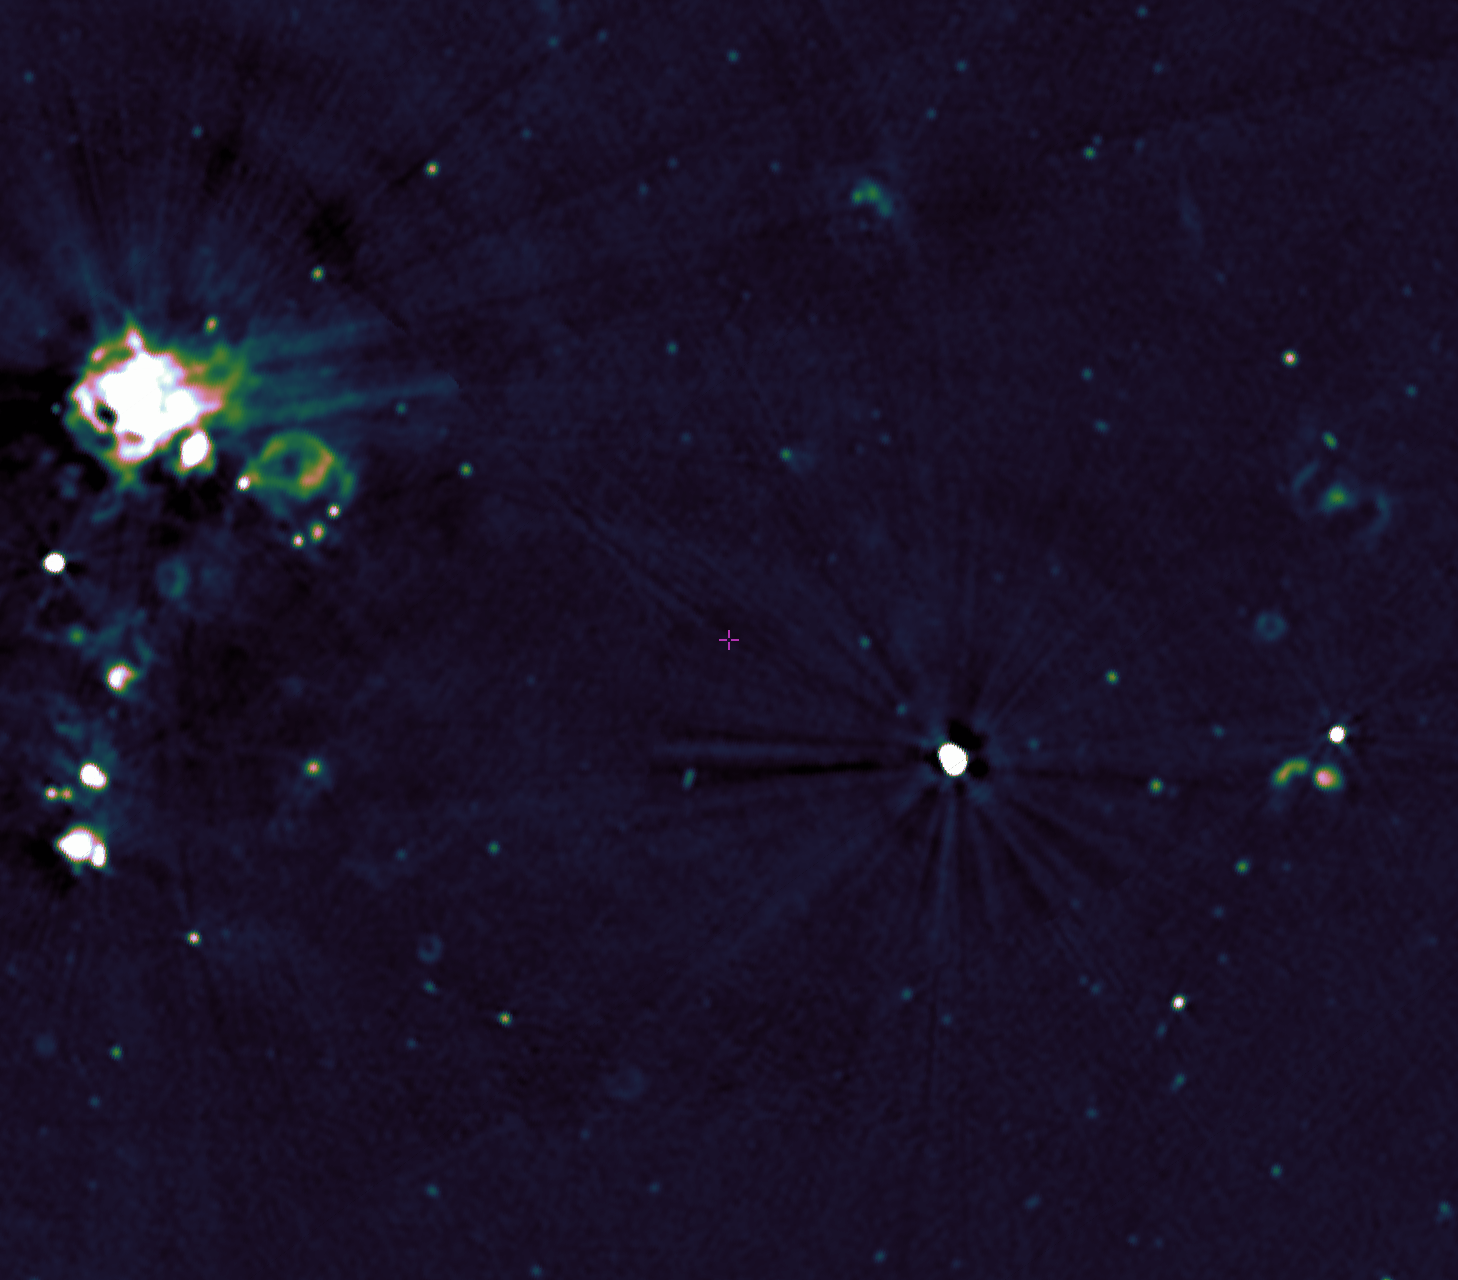
\includegraphics[width=1.0\linewidth]{./chapters/10.results/LMC/radio-843_cut.png}
		\caption{Radio wavelength at 843MHz.}
		\label{results:LMC:radio}
	\end{subfigure}
	\begin{subfigure}[b]{0.375\linewidth}
		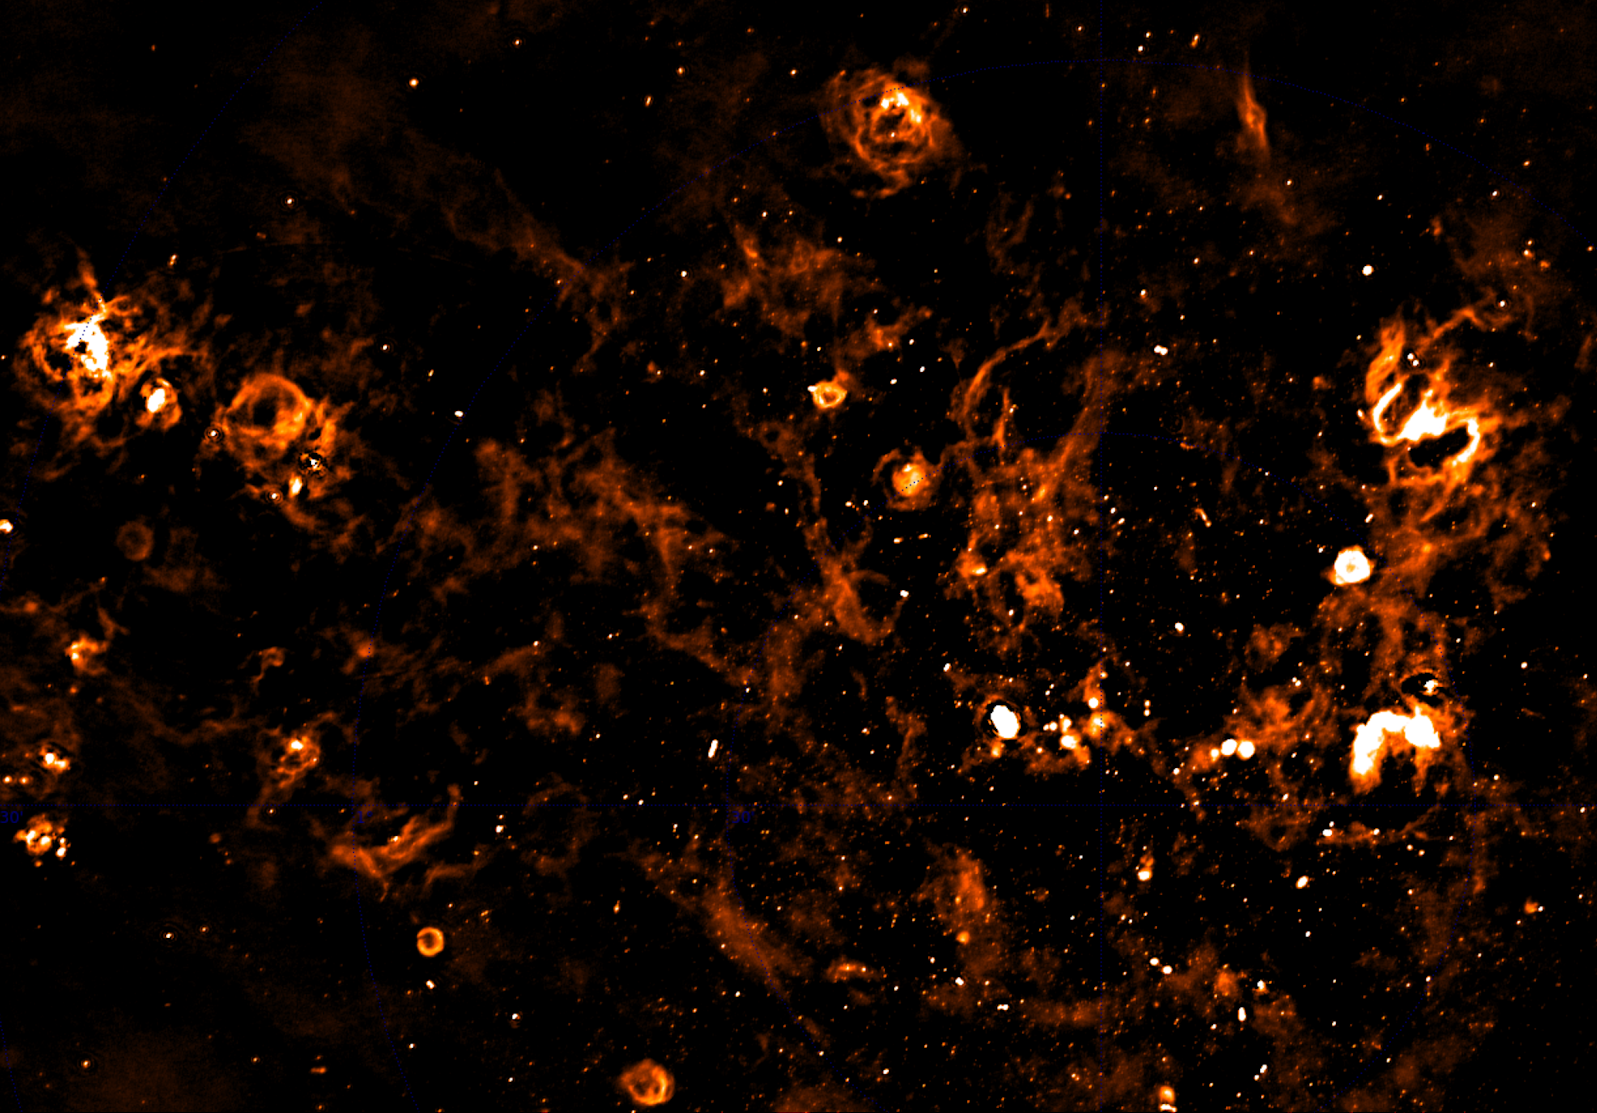
\includegraphics[width=1.0\linewidth]{./chapters/10.results/LMC/meerkat2.png}
		\caption{Wide band radio image by MeerKAT.}
		\label{results:LMC:meerkat}
	\end{subfigure}
	\caption{Large Magellanic Cloud (LMC)}
	\label{results:LMC}
\end{figure}

The MeerKAT observation covers a wide band of radio frequencies. The lowest frequency in the MeerKAT observation is 894 MHz, and the highest frequency is
Imaging the whole frequency band requires a wide band deconvolution algorithm. In wide band imaging, several images at different frequencies get deconvolved as an image cube. Wide band imaging again multiplies the amount of work that has to be done for reconstruction, as now we cannot deconvolve a single image, but have to deal with a whole image cube.

Wide band imaging is not possible within the time frame of this project. We take a narrow band subset of 5 channels from the original data (ranging from 1084 to 1088 MHz, about 1 Gb in size). 
Image section.

\begin{figure}[h]
	\centering
	\begin{subfigure}[b]{0.4\linewidth}
		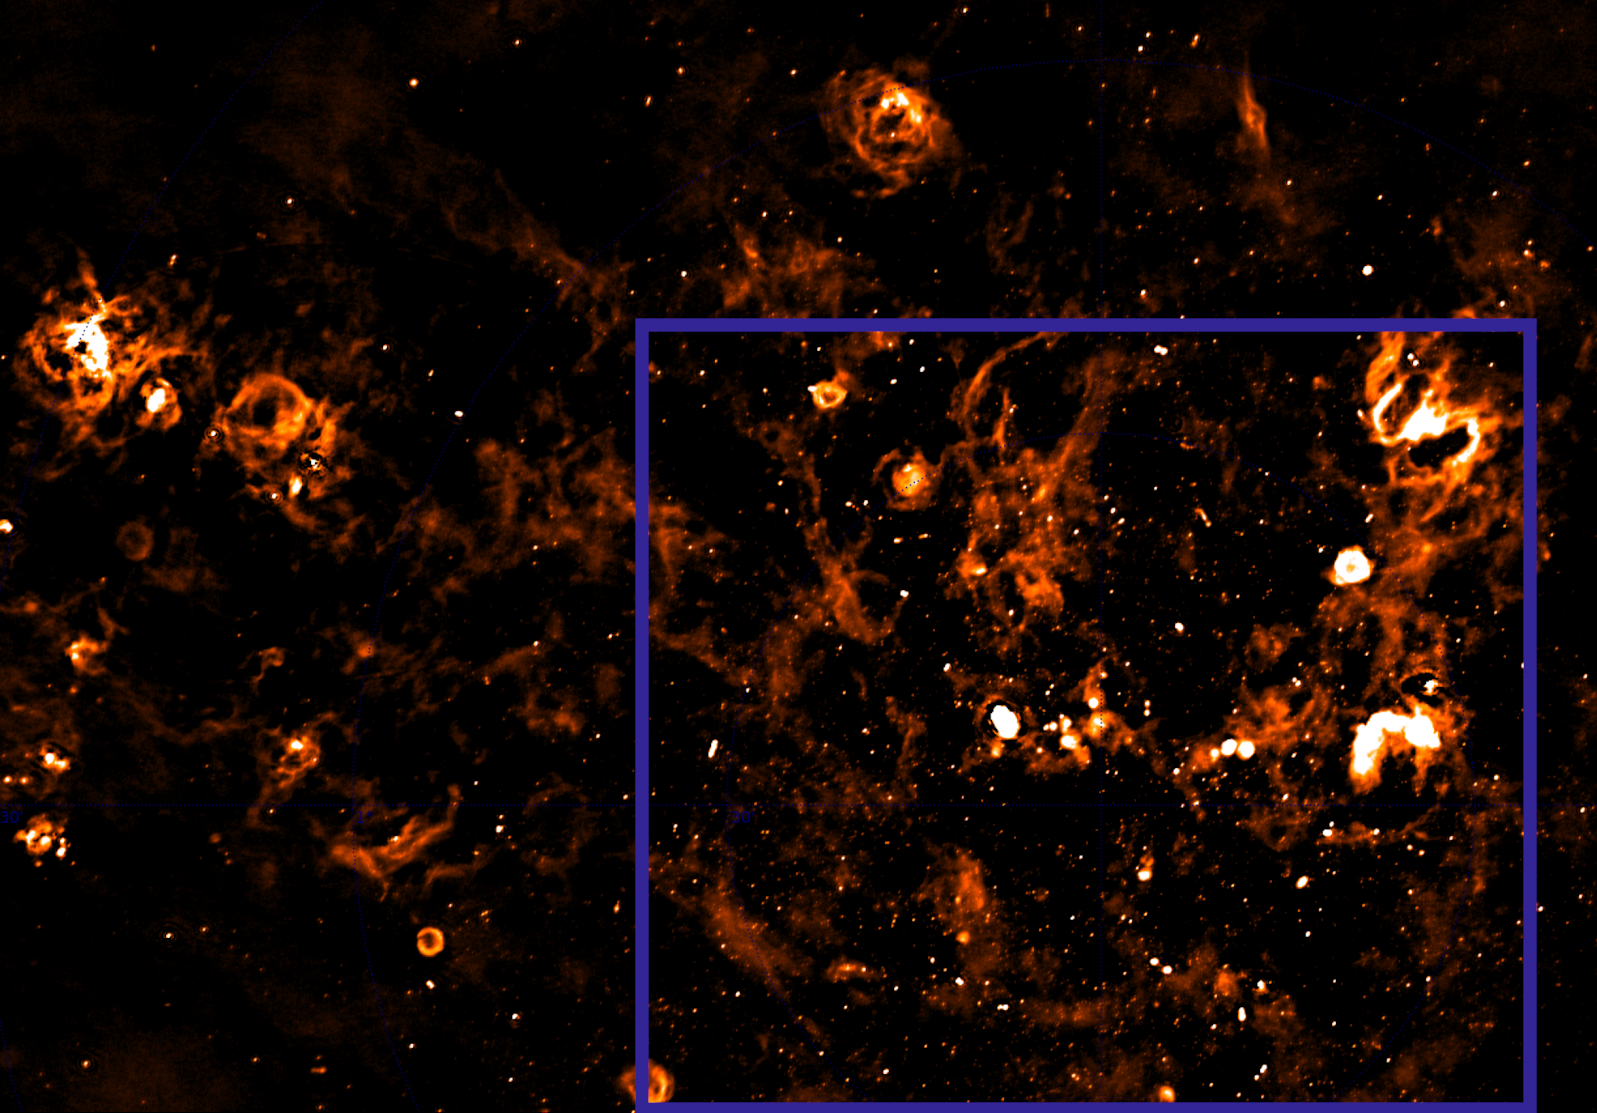
\includegraphics[width=1.0\linewidth]{./chapters/10.results/LMC/meerkat_cutout.png}
	\end{subfigure}
	\begin{subfigure}[b]{0.30\linewidth}
		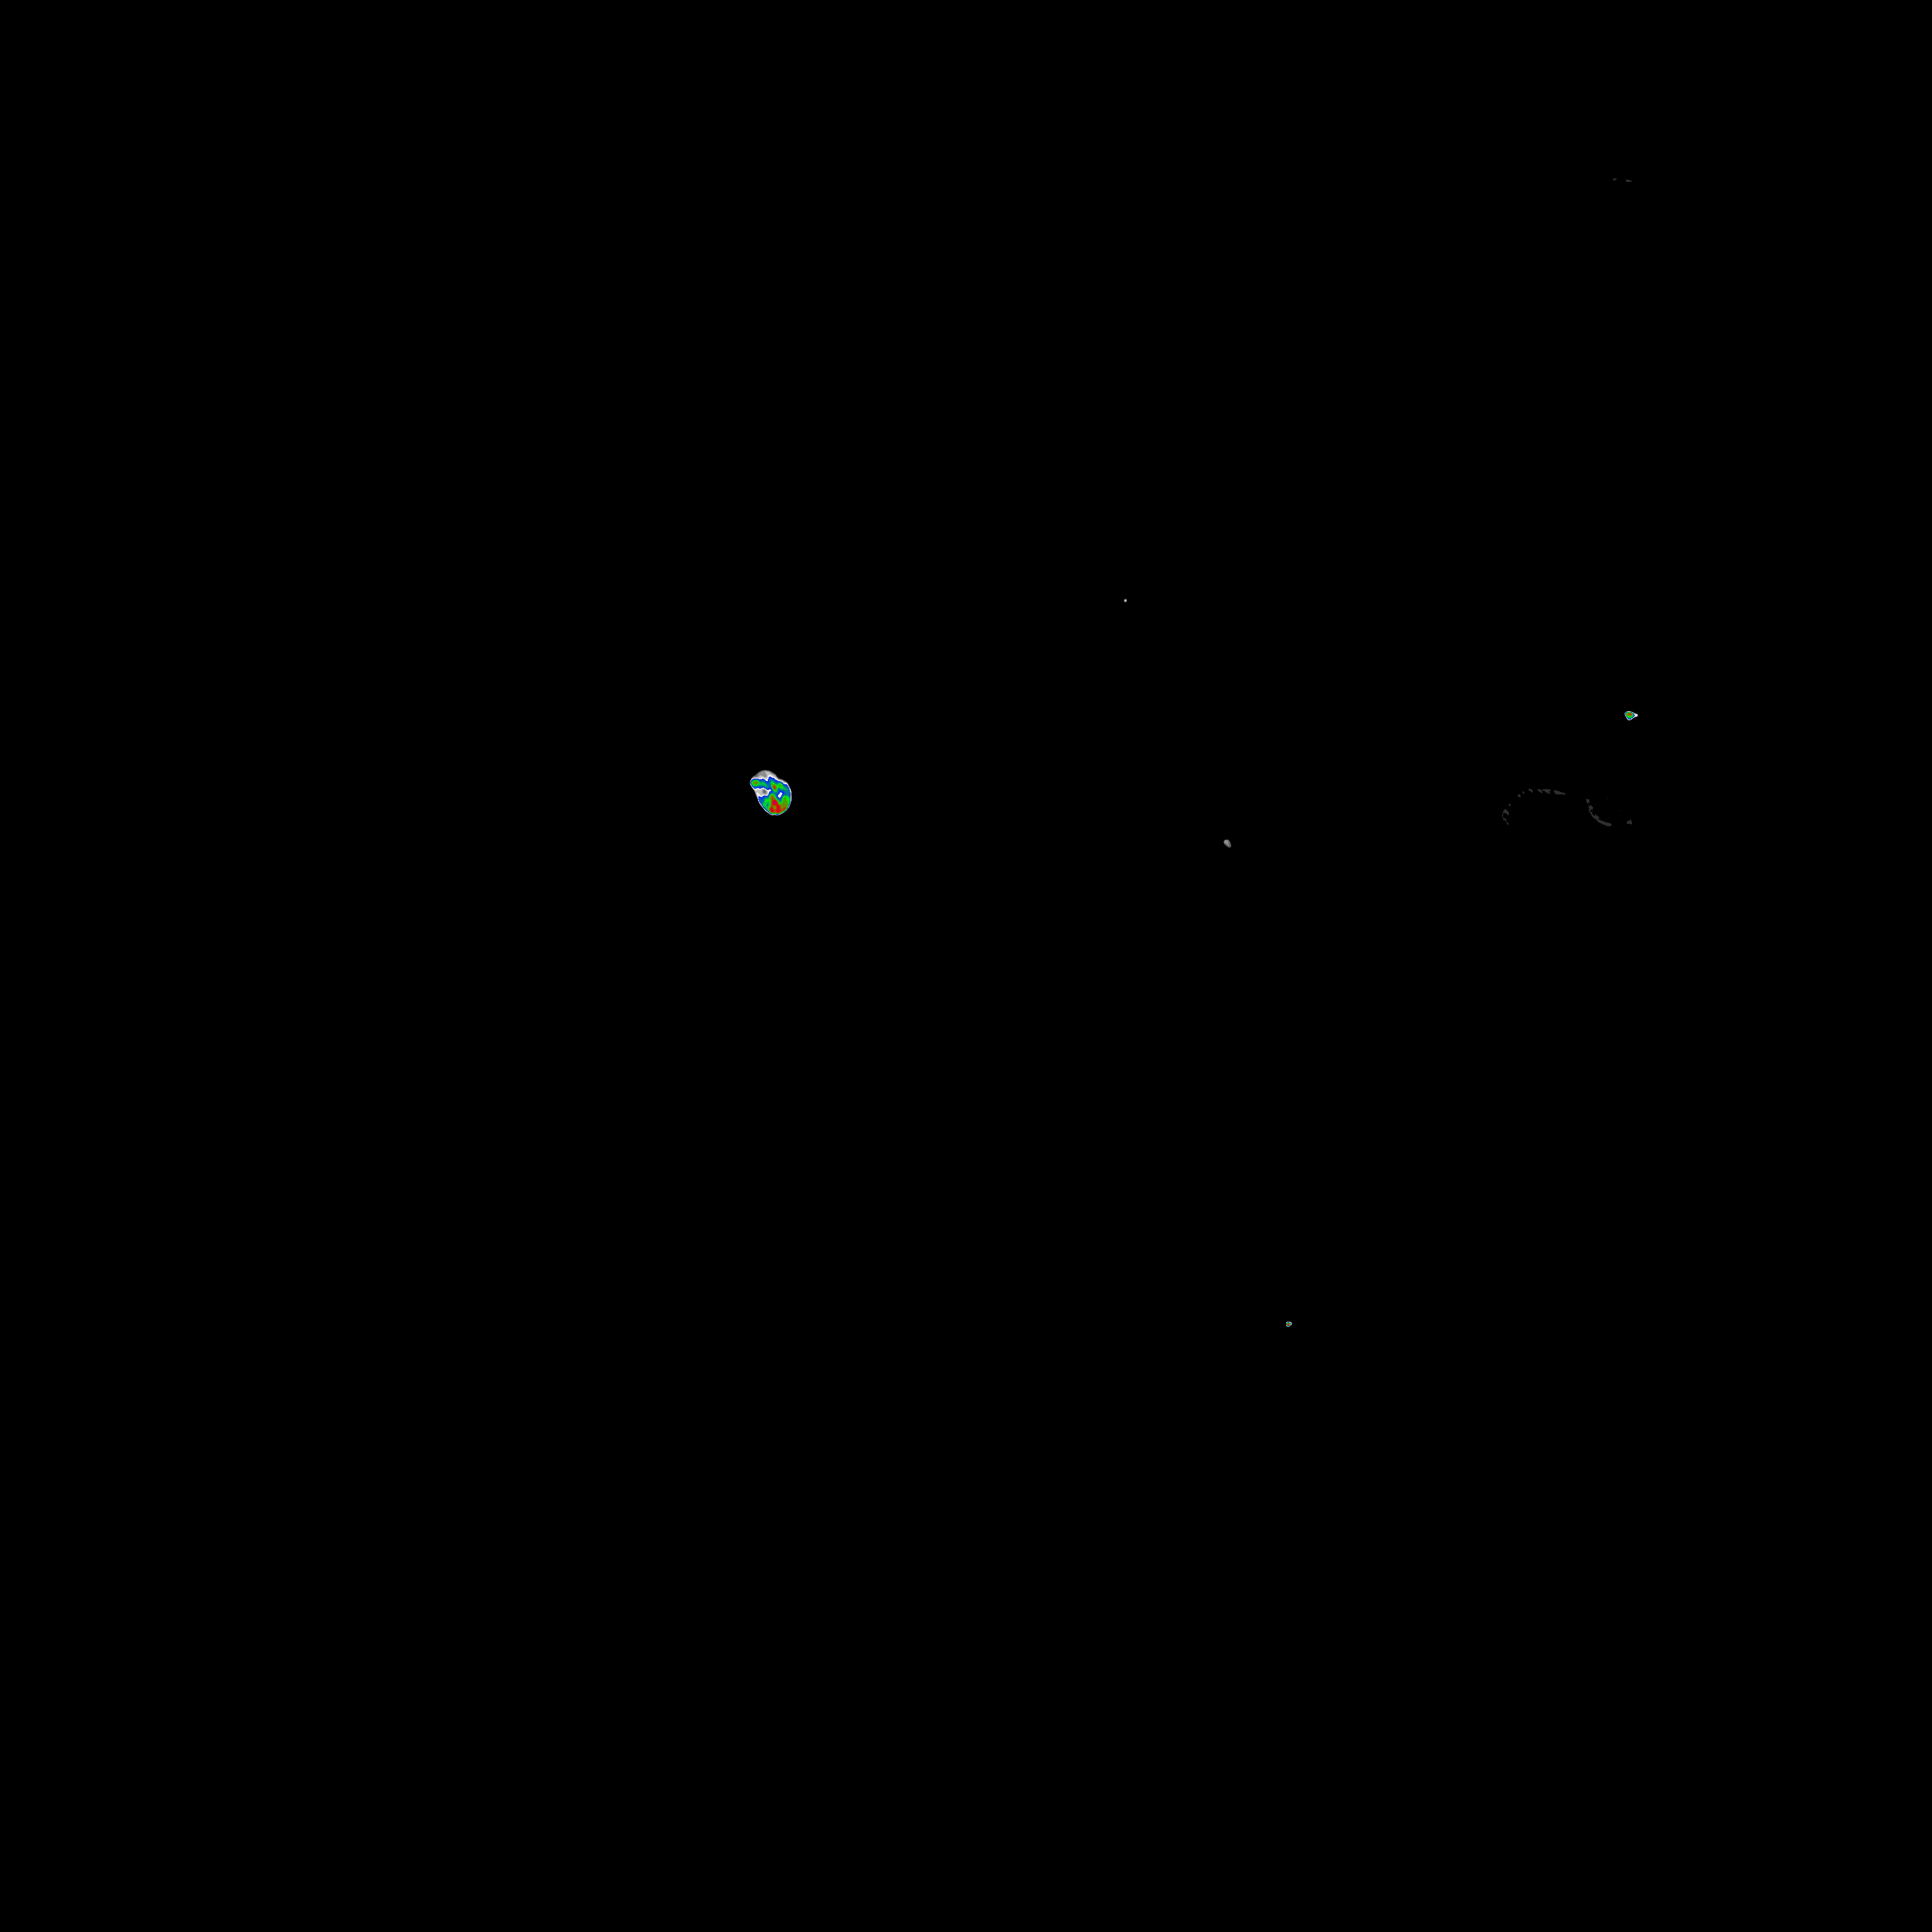
\includegraphics[width=1.0\linewidth]{./chapters/10.results/cleancomp/cd.png}
	\end{subfigure}
	\caption{Narrow band image section used.}
	\label{results:cutout}
\end{figure}

Wide field of view, correction of the w-term.

We use the subset to validate our coordinate descent deconvolution algorithm against CLEAN in Section \ref{results:cleancomp}.
We then test if we can do the proper parallel reconstruction.



The LMC is already a difficult field to reconstruct.


Interpolation between the frequencies
Wideband adds a lot more faint structures in the image.
Huge amount of non-zero pixels, puts a strain on the deconvolution algorithm.
The image was reconstructed with multi-frequency-synthesis CLEAN.
Wide-band imaging Cube of data. 

LMC is a difficult field to reconstruct. we require both wide band and wide-field-of-view imaging for an accurate reconstruction. 









We cannot do wide-band imaging with our proof-of-concept algorithm. We can correct for the $w$-term, but cannot image wide-band. imaging
Wideband imaging would need this: several deconvolution steps at different frequencies, and interpolation between them.
Data size, we need to image a cube of data.

Out of scope for this project. We do not handle this.


We use a 1 GB subset of the original observation. We image 5 channels over a bandwidth of ()
use a smaller section of the image

First, we compare the image we reconstruct
See how much we can use with GPU-acceleration and a naive way to distribute things.


\subsection{Comparison with CLEAN reconstruction} \label{results:cleancomp}

Wide field, but

Imaging parameters
WSCLEAN was used for reconstruction. Multiscale.




\begin{figure}[h]
	\centering
	\begin{subfigure}[b]{0.4\linewidth}
		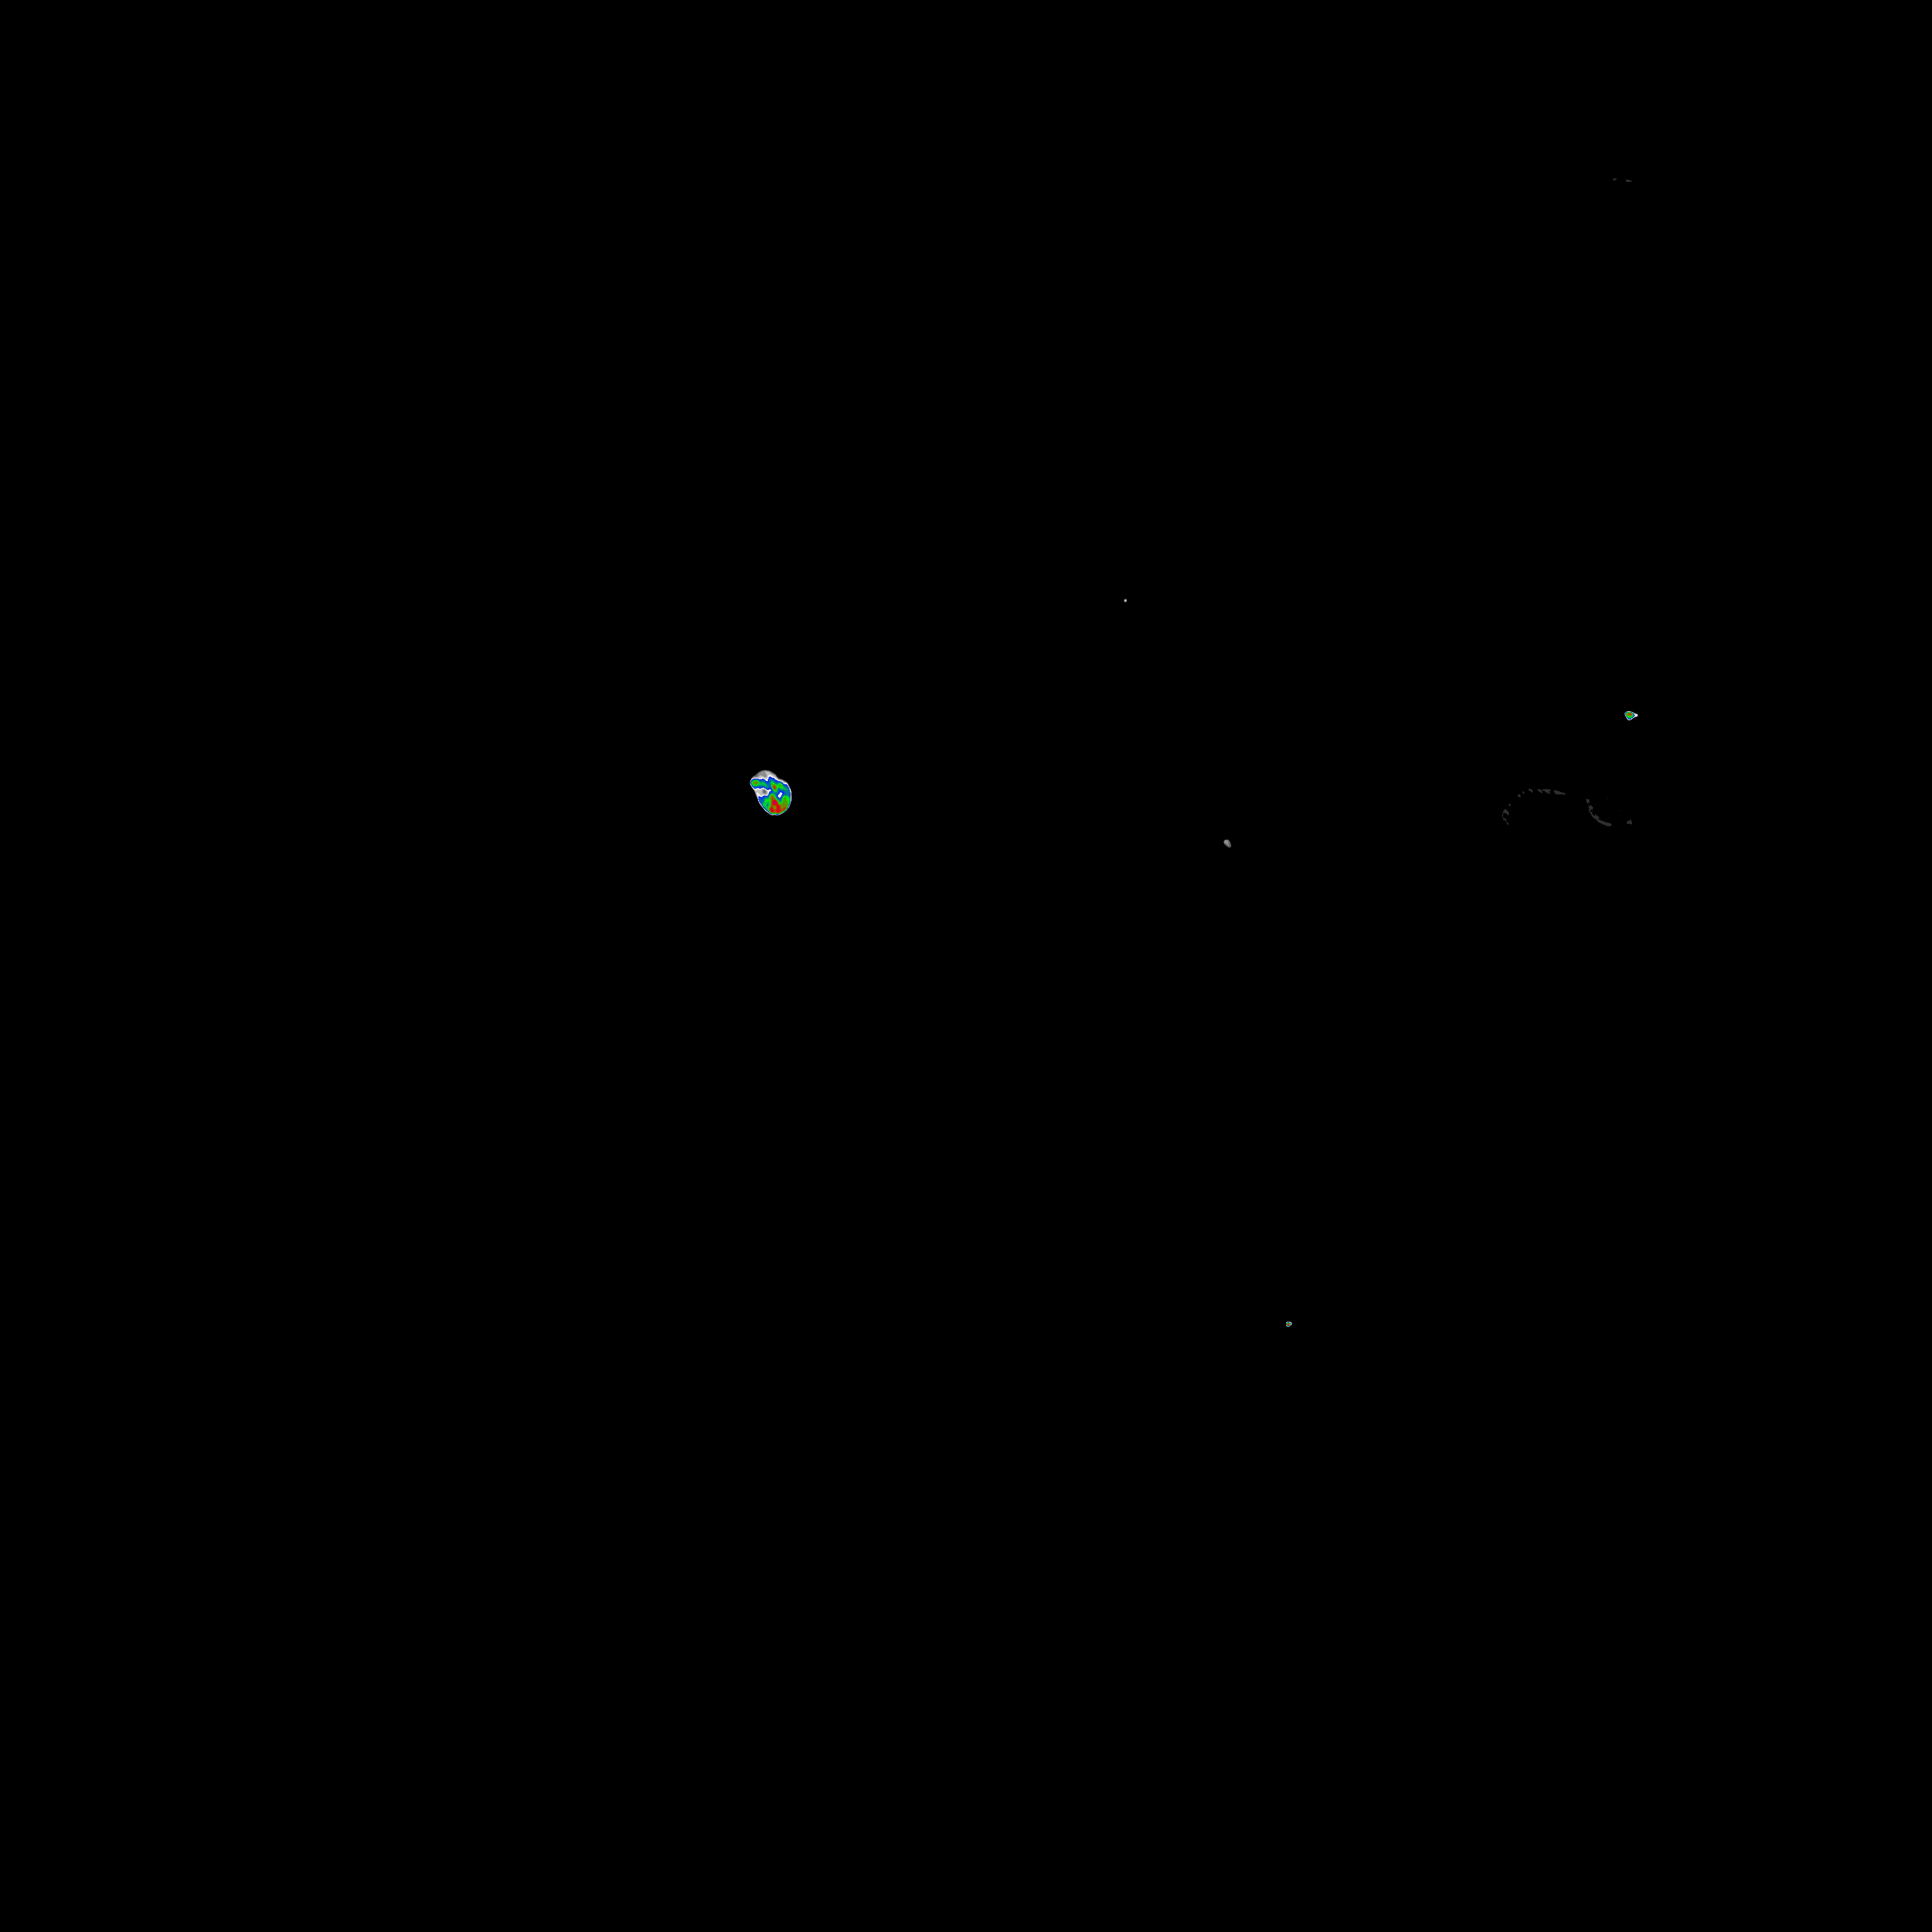
\includegraphics[width=1.00\linewidth]{./chapters/10.results/cleancomp/cd.png}
		\caption{Multiscale CLEAN reconstruction.}
		\label{results:comp:clean}
	\end{subfigure}
	\begin{subfigure}[b]{0.40\linewidth}
		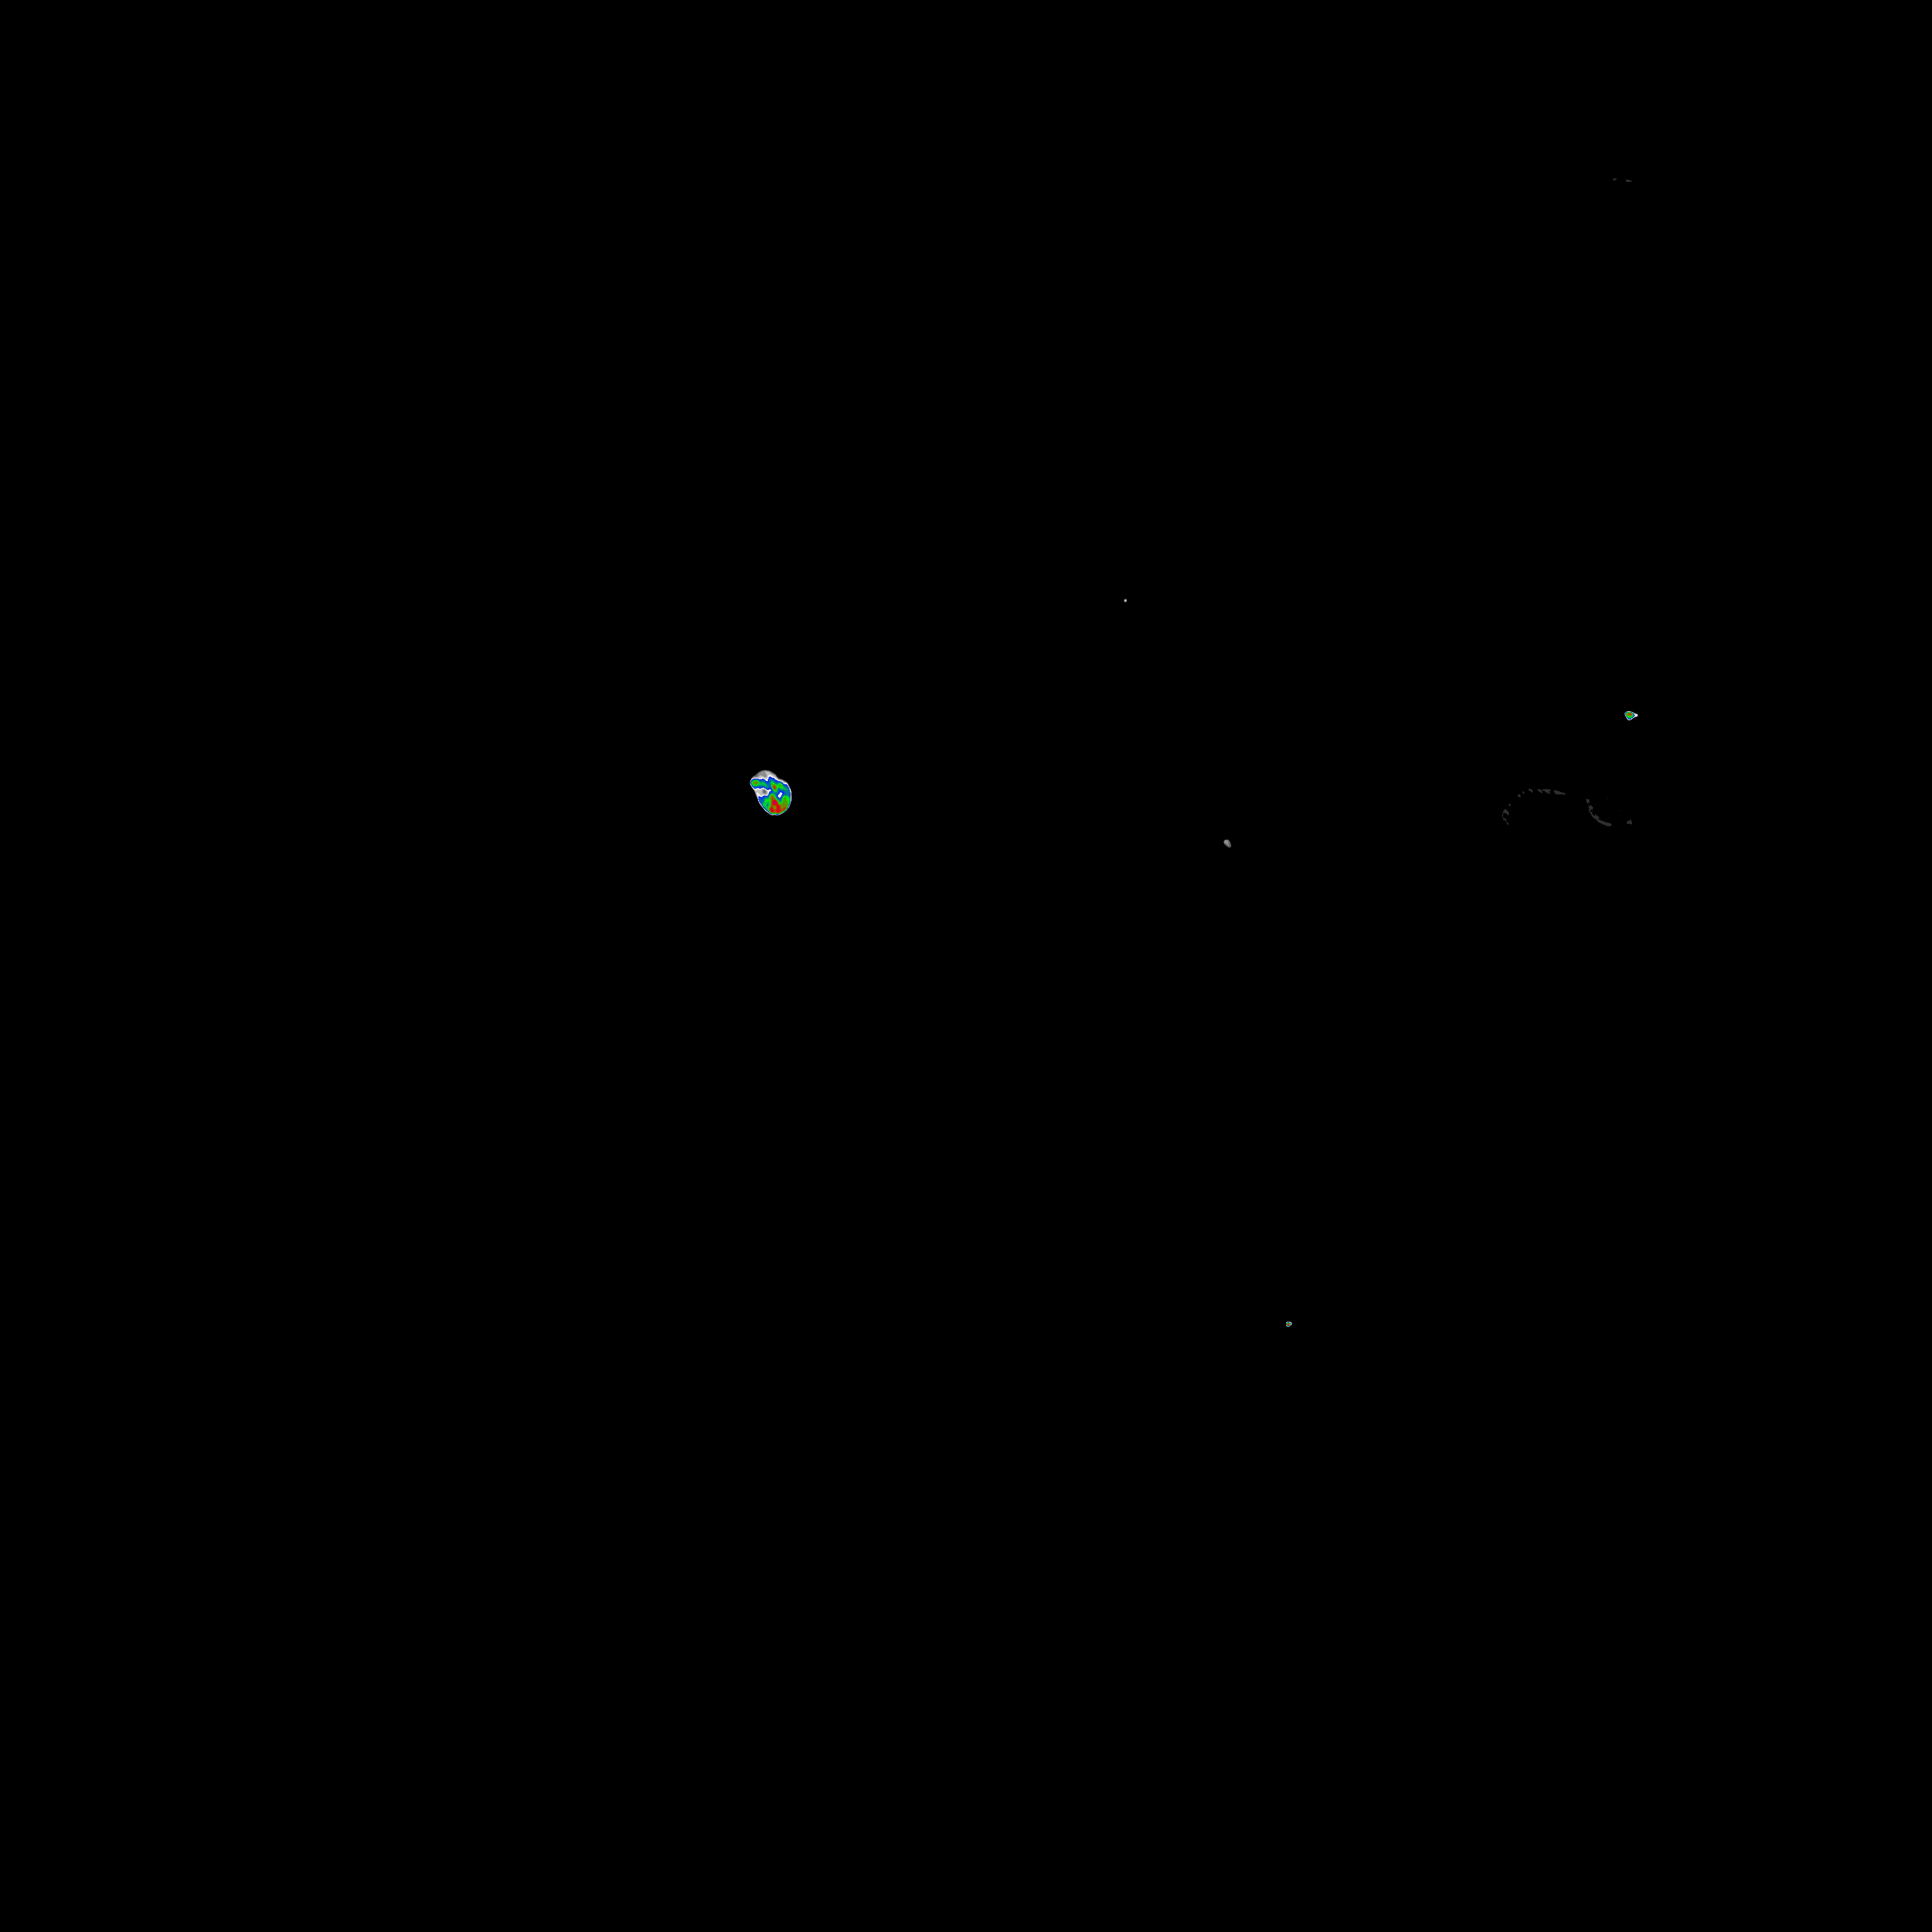
\includegraphics[width=1.00\linewidth]{./chapters/10.results/cleancomp/cd.png}
		\caption{Coordinate descent reconstruction.}
		\label{results:comp:cd}
	\end{subfigure}
	\caption{Speedup by using MPI or GPU acceleration}
	\label{results:cleancomp:figure}
\end{figure}

Numbers of Major cycles used by CLEAN.
Number of iterations

Number of Major cycles used by CD
number of iterations

Compare the N321D supernova remnant.

CLEAN with natural weighting.

CLEAN with briggs weighting. Narrower PSF than the CLEAN natural weighting reconstruction. As such, it finds more structures inside the supernova remnant.

Briggs is a weighting scheme of the visibilities. Commonly used in radio astronomy.
 improves PSF.
 Not implemented in our pipeline.
Coordinate descent deconvolution has to work with natural weighting.
But it

\begin{figure}[h]
	\centering
	\begin{subfigure}[b]{0.3\linewidth}
		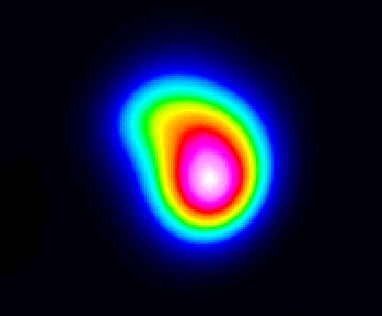
\includegraphics[width=1.00\linewidth]{./chapters/10.results/cleancomp/n132_clean.png}
		\caption{CLEAN Natural weighting.}
		\label{results:N132:clean}
	\end{subfigure}
	\begin{subfigure}[b]{0.3\linewidth}
		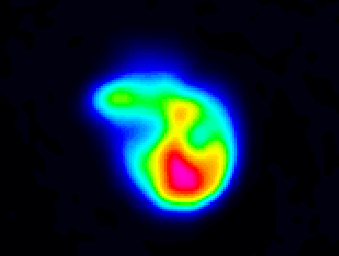
\includegraphics[width=1.00\linewidth]{./chapters/10.results/cleancomp/n132_clean_briggs.png}
		\caption{CLEAN Briggs weighting.}
		\label{results:N132:cleanbriggs}
	\end{subfigure}
	\begin{subfigure}[b]{0.3\linewidth}
		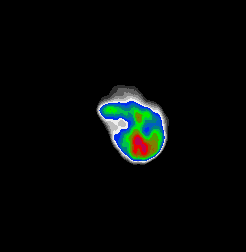
\includegraphics[width=1.00\linewidth]{./chapters/10.results/cleancomp/n132_cd.png}
		\caption{CD Natural weighting.}
		\label{results:comp:N132:cd}
	\end{subfigure}
	\caption{N132 comparison}
	\label{results:cleancomp::N132:figure}
\end{figure}

Approximation of the gradient update step works

Comparable to clean.
It works.


\subsection{Coordinate descent acceleration with MPI or GPU}

Describe hardware

Distributed with MPI

GPU implementation

Measurement of the speedup.

\begin{figure}[h]
	\centering
		\begin{subfigure}[b]{0.4\linewidth}
		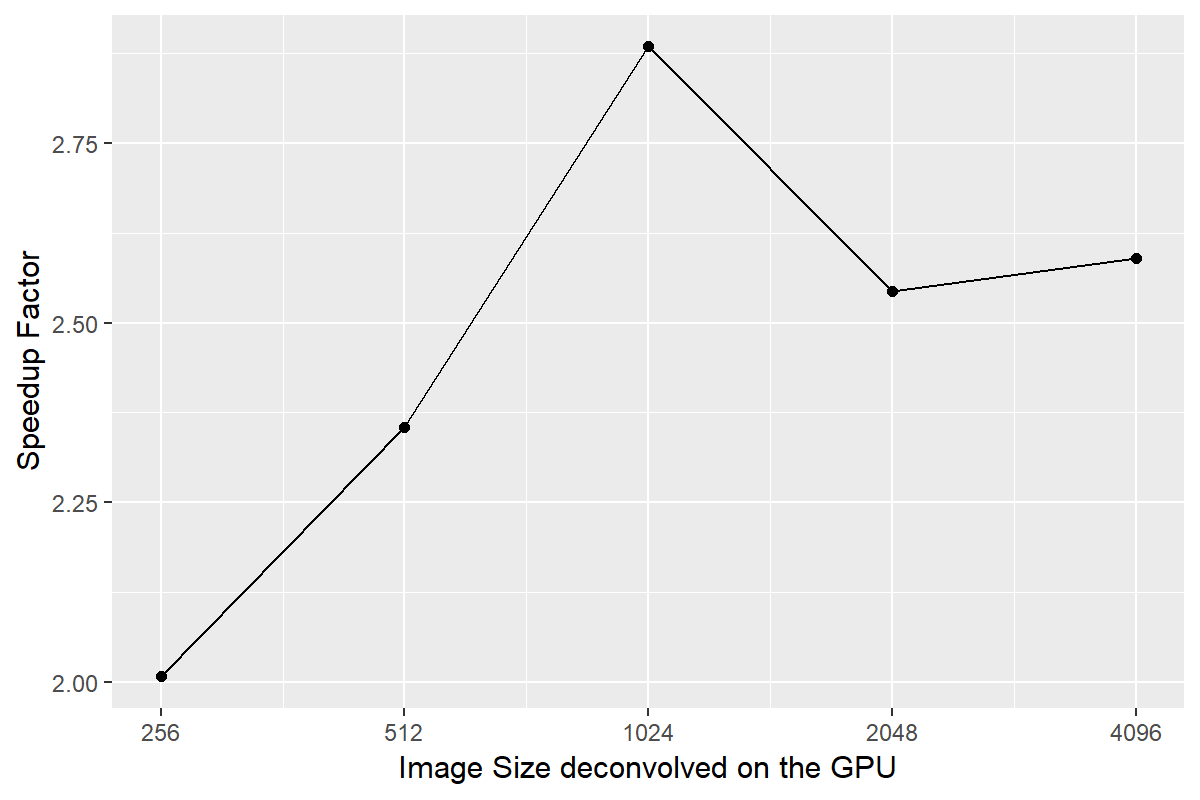
\includegraphics[width=1.00\linewidth]{./chapters/10.results/speedup/gpu.png}
	\end{subfigure}
	\begin{subfigure}[b]{0.4\linewidth}
		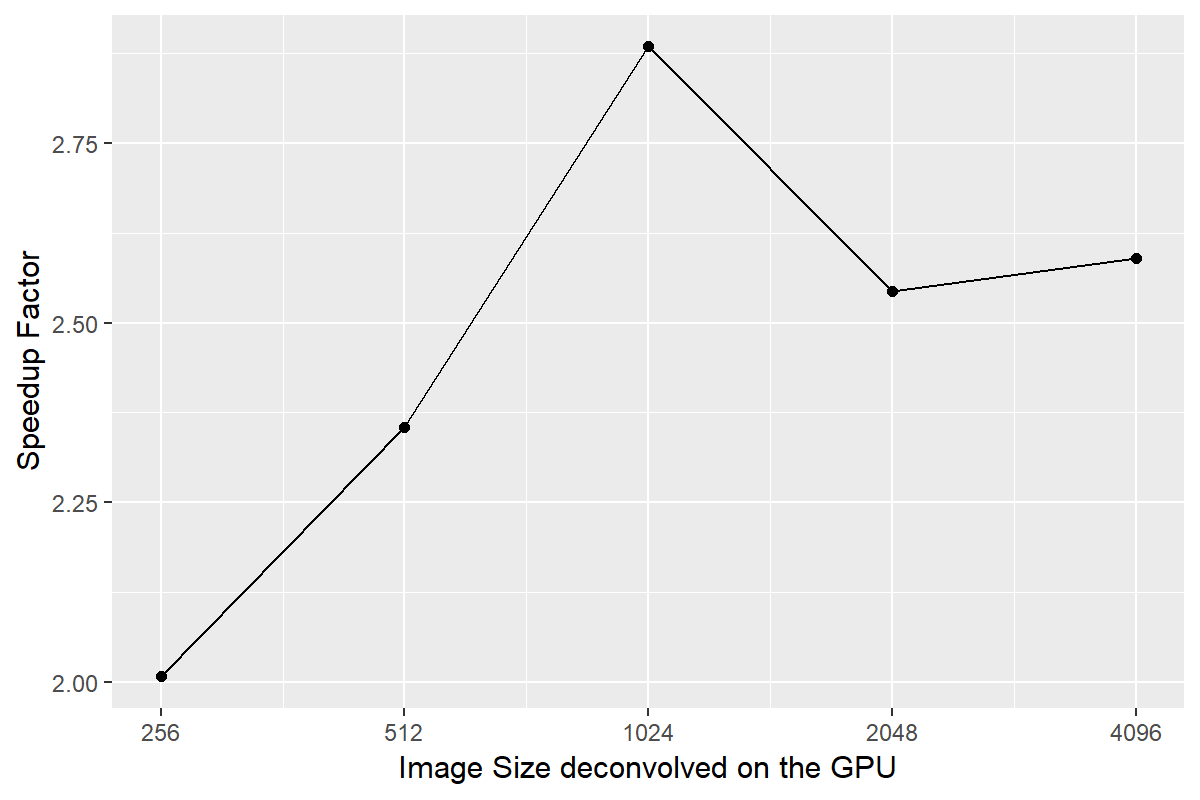
\includegraphics[width=1.00\linewidth]{./chapters/10.results/speedup/gpu.png}
	\end{subfigure}
	\caption{Speedup by using MPI or GPU acceleration}
	\label{results:speedup}
\end{figure}


We cannot use MPI combined with the GPU. The MPI implementation uses a communication step in each coordinate descent iteration (communicating which pixel to optimize with MPI Allreduce). 



\subsection{Effect of approximating the $PSF$} \label{results:gradients}
can we reduce the $PSF$

\begin{figure}[h]
	\centering
	\begin{subfigure}[b]{0.6\linewidth}
		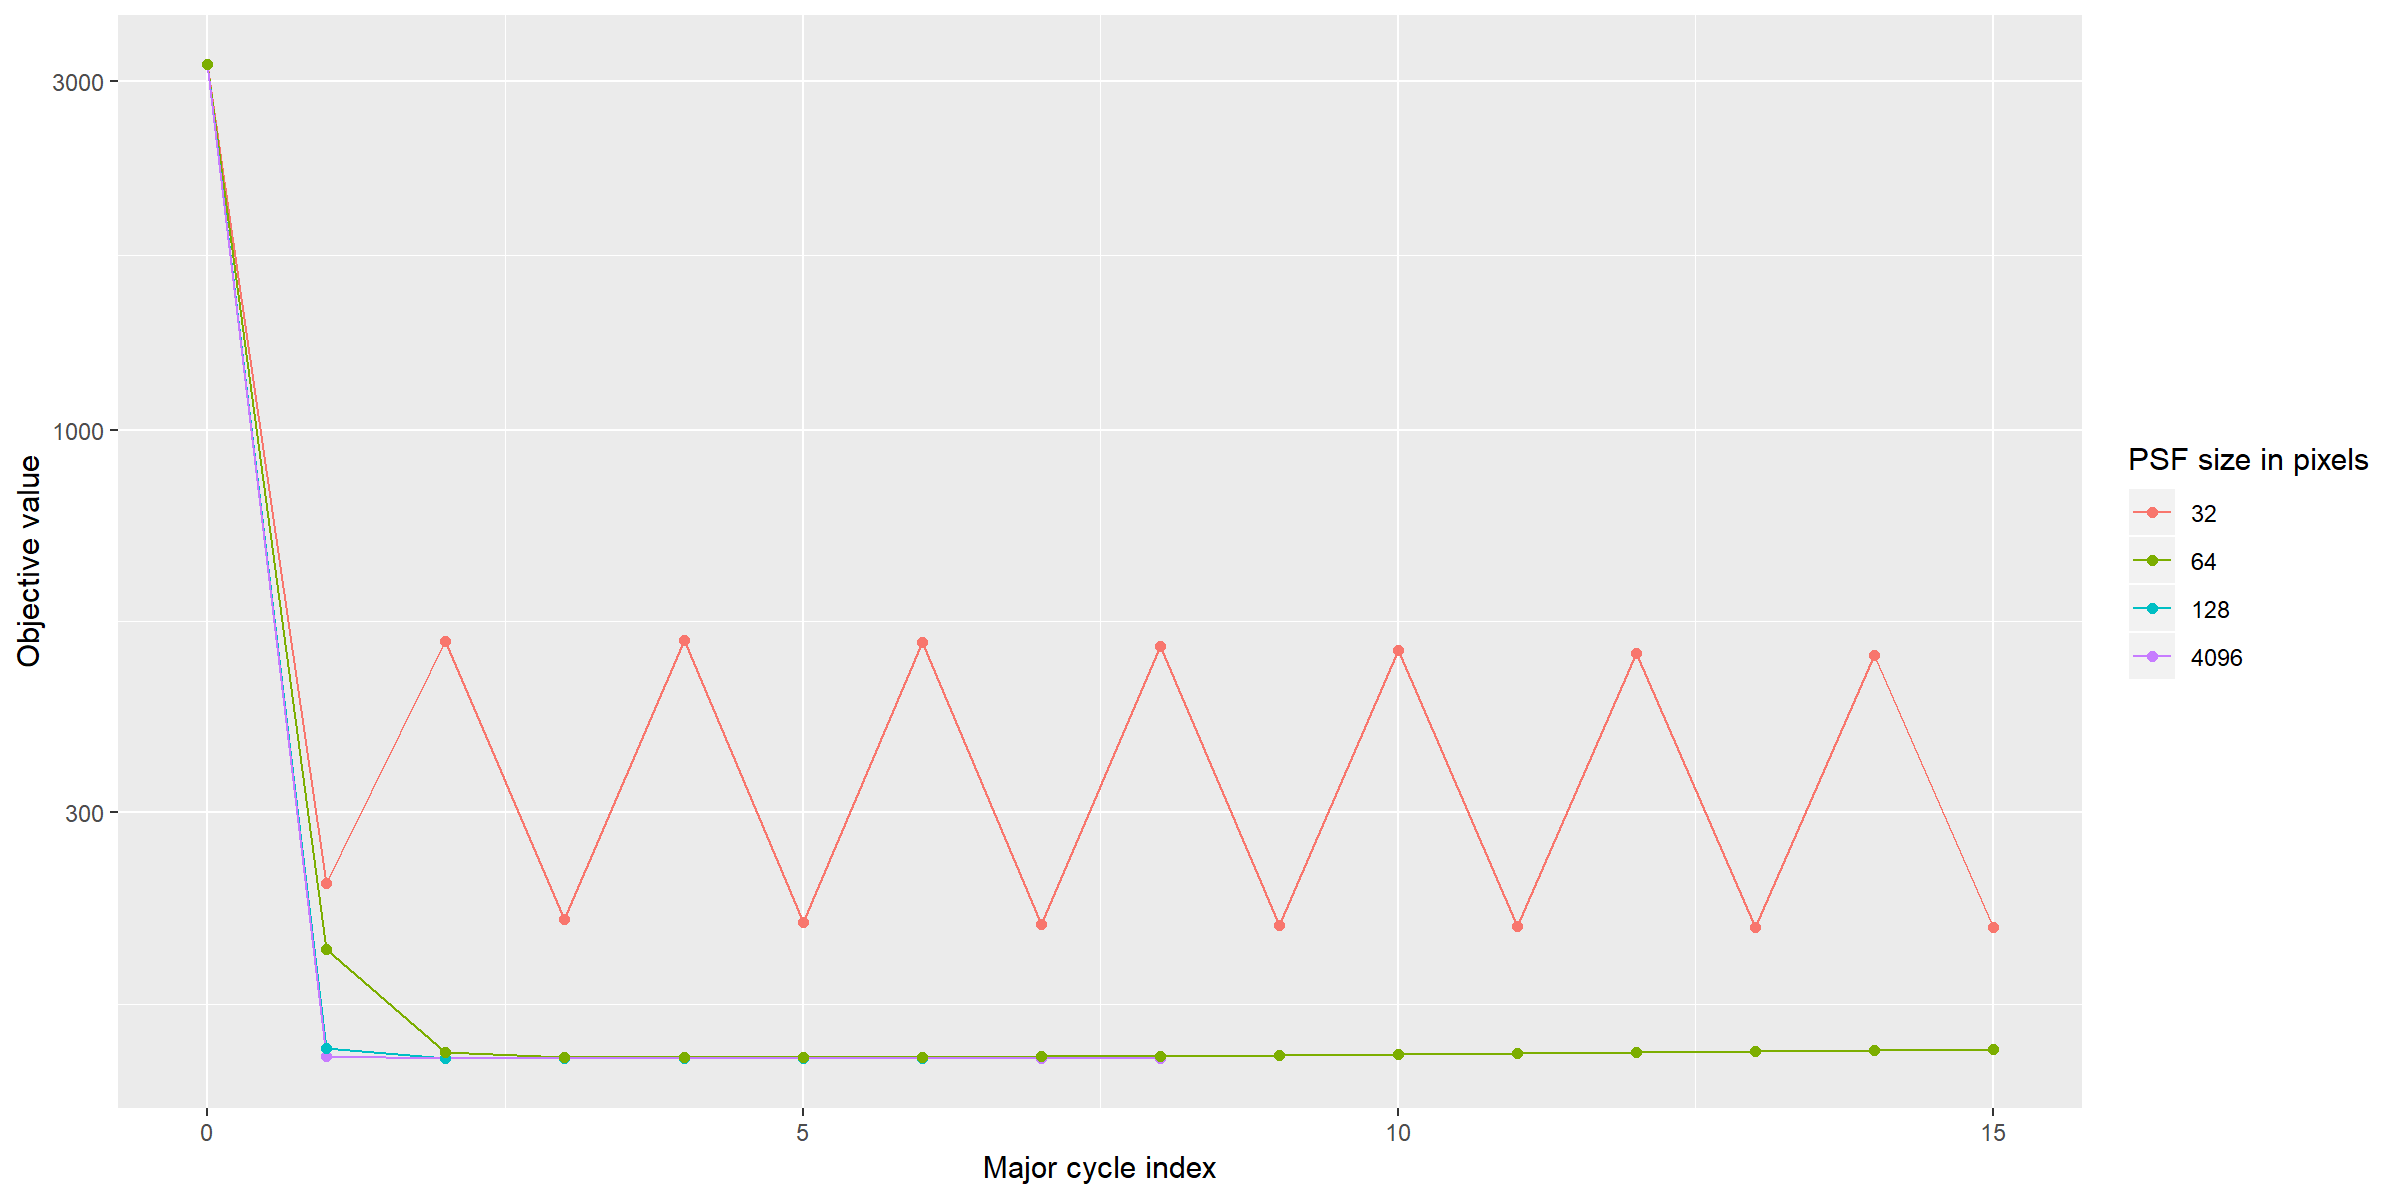
\includegraphics[width=\linewidth]{./chapters/10.results/gradient/size.png}
	\end{subfigure}
	\begin{subfigure}[b]{0.36\linewidth}
		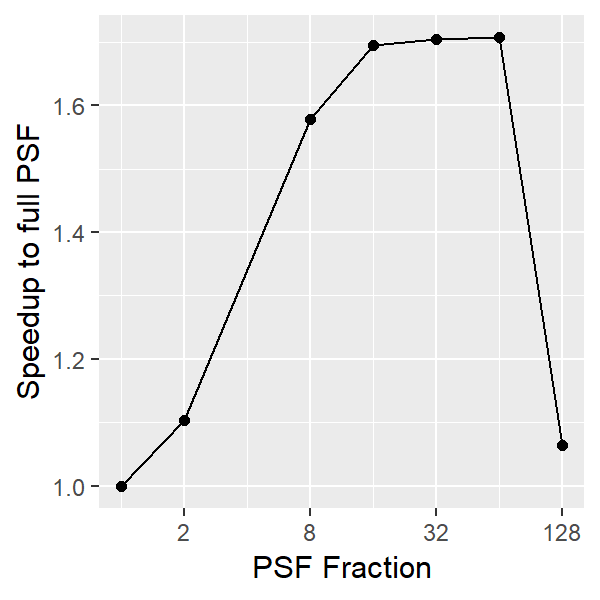
\includegraphics[width=\linewidth]{./chapters/10.results/gradient/speedup.png}
	\end{subfigure}
	
	\caption{Effect of the L1 and L2 Norm separately.}
	\label{results:gradients:size}
\end{figure}

\begin{figure}[h]
	\centering
	\begin{subfigure}[b]{1.0\linewidth}
		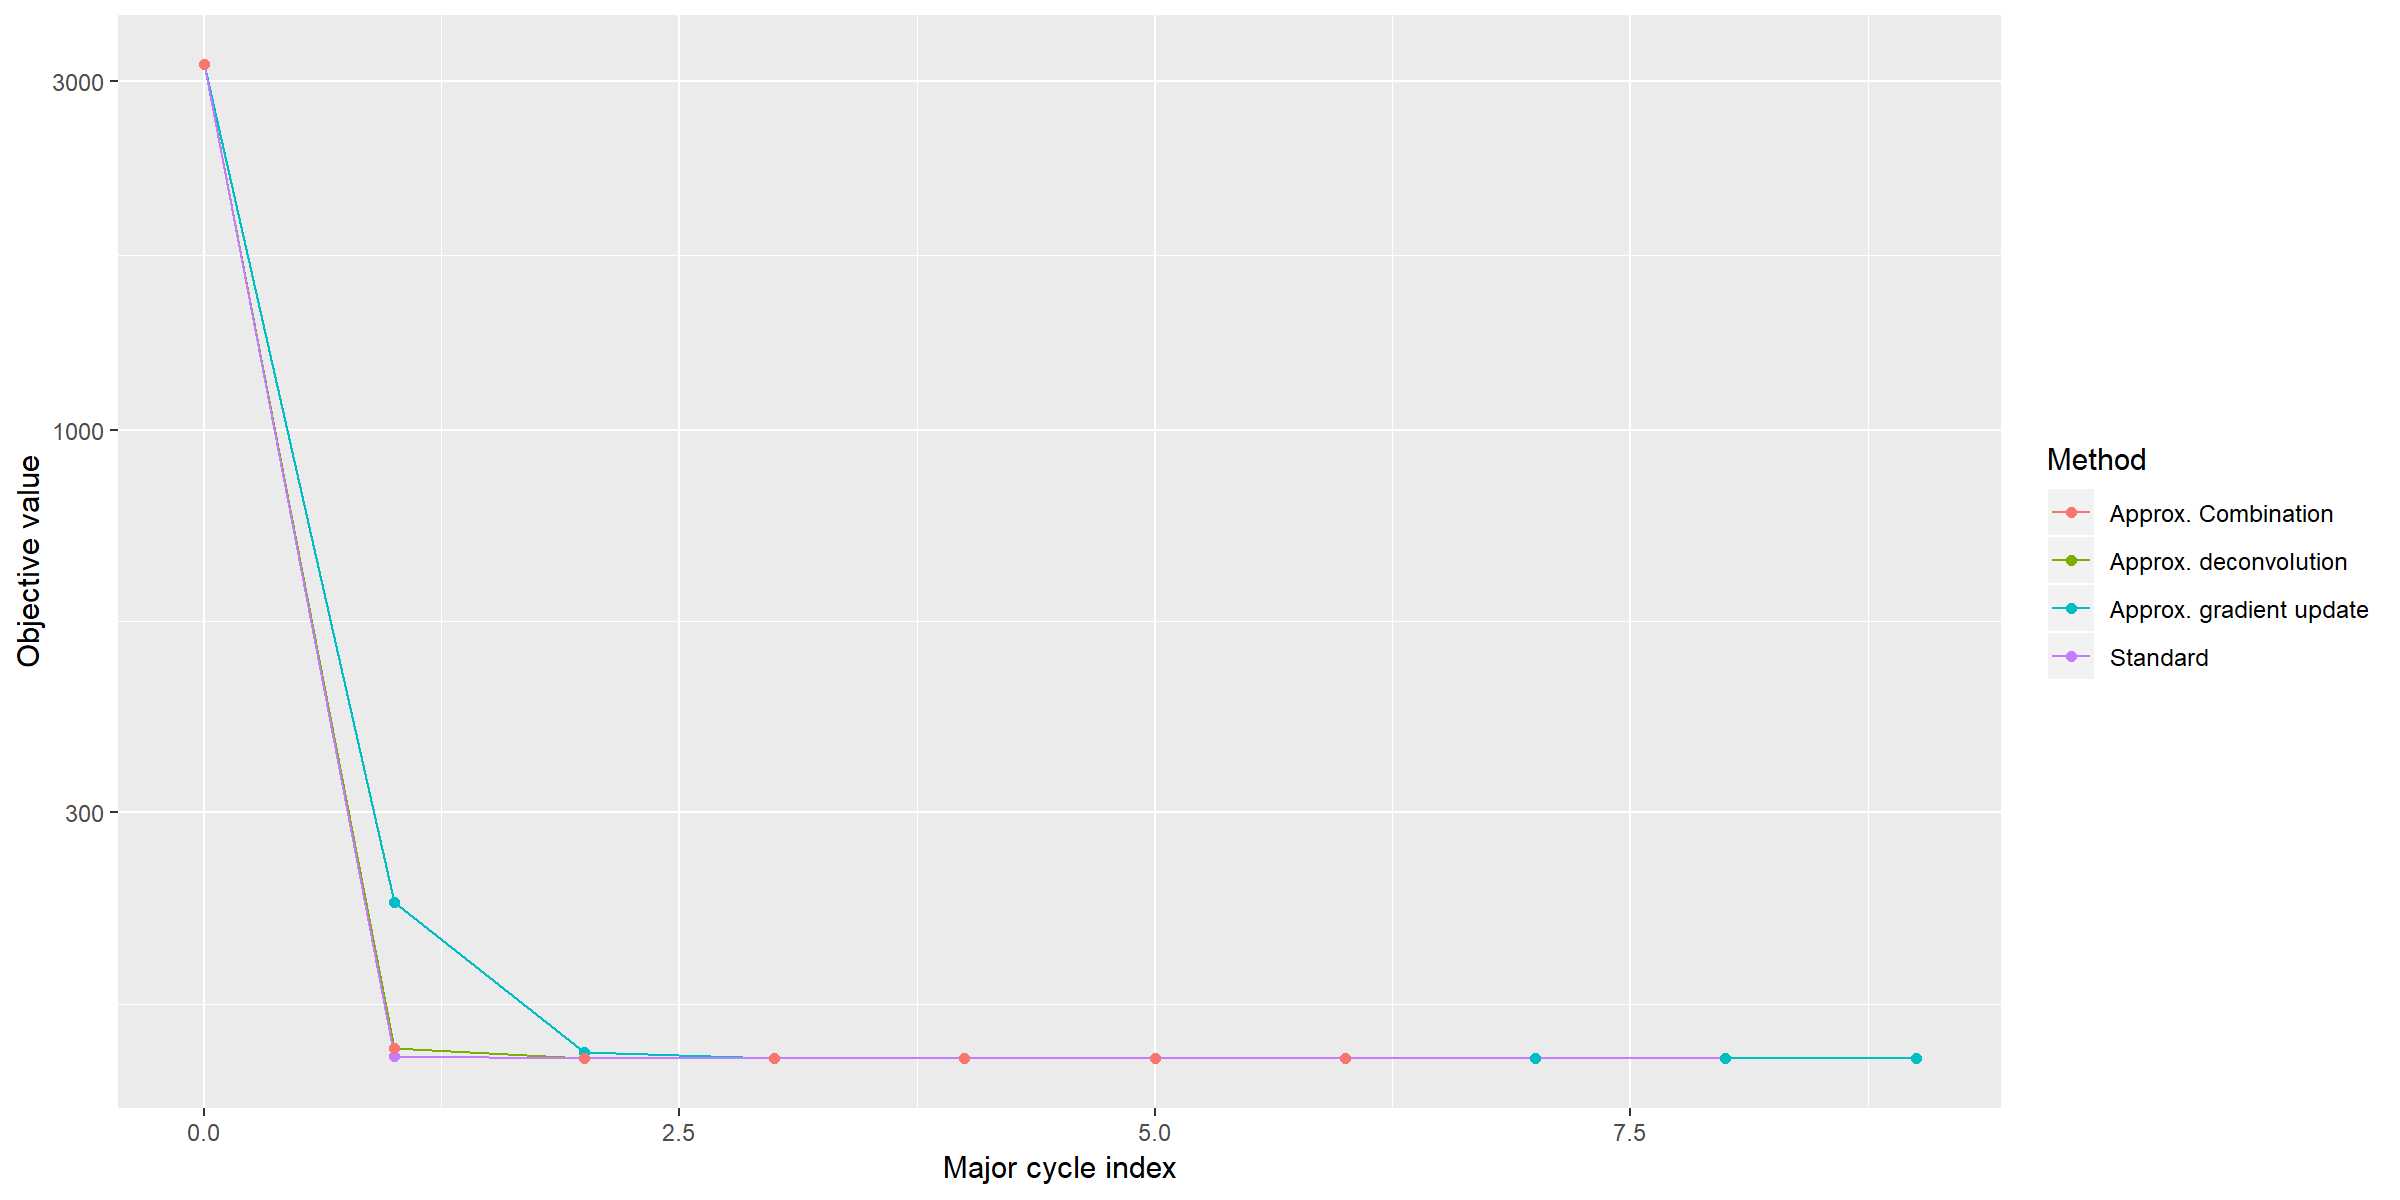
\includegraphics[width=\linewidth]{./chapters/10.results/gradient/comparison.png}
	\end{subfigure}
	\begin{subfigure}[b]{1.0\linewidth}
		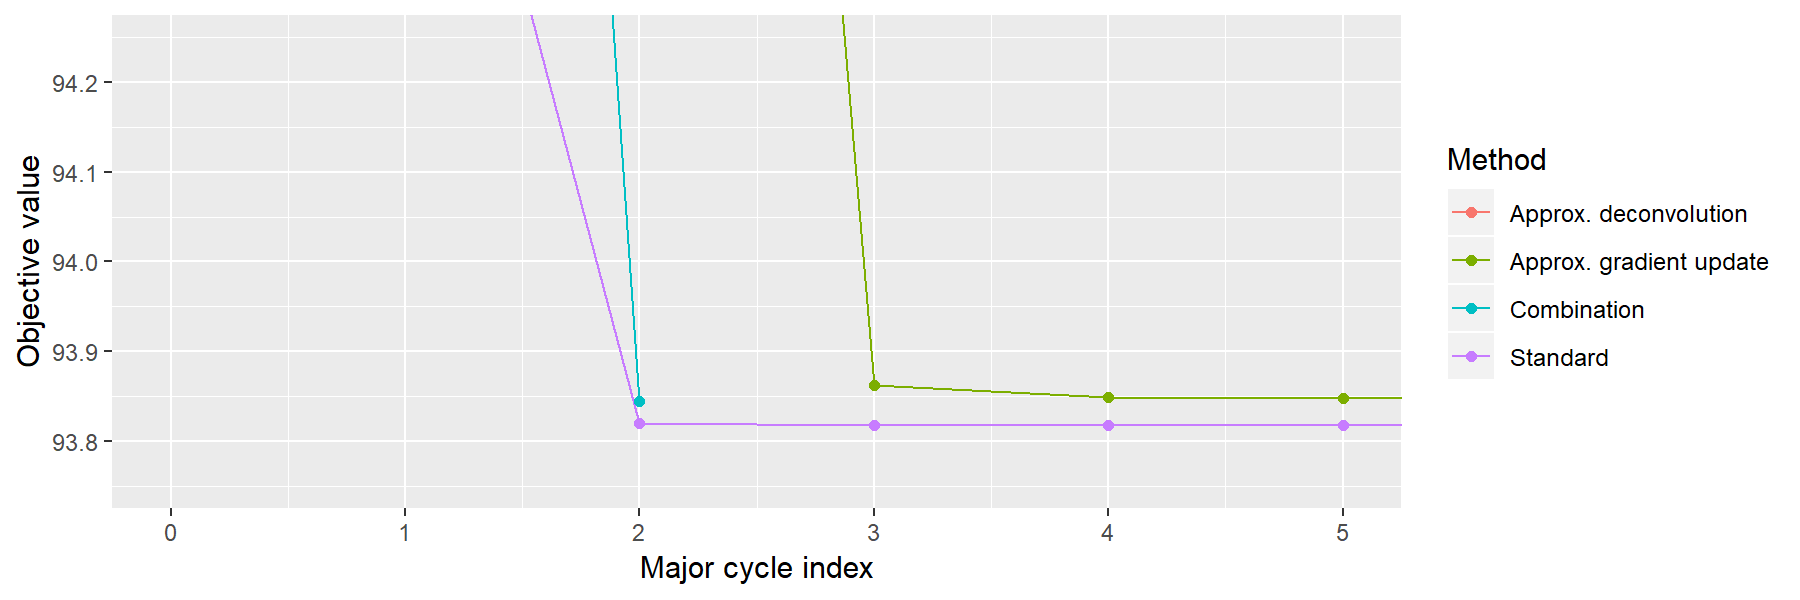
\includegraphics[width=\linewidth]{./chapters/10.results/gradient/comparison_zoom.png}
	\end{subfigure}
	
	\caption{Effect of the L1 and L2 Norm separately.}
	\label{results:gradients:comparison}
\end{figure}